\documentclass{sig-alternate-05-2015}

\usepackage{url}                  % format URLs
\usepackage{listings}          % format code
\lstset{
  mathescape, 
  language={C},
  basicstyle=\small
}
\usepackage{enumitem}      % adjust spacing in enums
\usepackage[colorlinks=true,allcolors=blue,breaklinks,draft=false]{hyperref}   
\usepackage{graphicx}
\usepackage{float,subfig}
\usepackage{xspace,framed}
\usepackage{colortbl}
\usepackage{calc}
\usepackage[dvipsnames]{xcolor}

\usepackage{algorithm}
\usepackage{amsfonts}
\usepackage{multicol}
\usepackage{multirow}
\usepackage{tikz}
\usetikzlibrary{positioning, automata, shapes.arrows, calc, shapes, arrows}
\usepackage[justification=centering]{caption}
\usepackage{stmaryrd}
\usepackage{hhline}
\usepackage{pifont}
\usepackage{longtable}
\usepackage{afterpage}
\usepackage{wasysym}
%\usetikzlibrary{decorations}
%\usetikzlibrary{decorations.pathmorphing}

\newcommand{\blue}[1]{{\color{blue}#1}}
\newcommand{\red}[1]{{\color{red}#1}}
\newcommand{\green}[1]{{\color{green}#1}}

\newtheorem{myassumption}{Assumption}
\newtheorem{mylemma}{Lemma}

\newcommand{\lcsay}[1]{{\color{Magenta} LC: {#1}}} 
\newcommand{\dcsay}[1]{{\color{purple} DC: {#1}}}
\newcommand{\dksay}[1]{{\color{blue} DK: {#1}}}  
\newcommand{\aasay}[1]{{\color{red} AA: {#1}}} 
\newcommand{\cdsay}[1]{{\color{Mahogany} CD: {#1}}} 
\newcommand{\pksay}[1]{{\color{RoyalBlue} PK: {#1}}} 
\newcommand{\ibsay}[1]{{\color{Sepia} IB: {#1}}} 

\newcommand{\param}[2]{\ensuremath{\langle{#1},{#2}\rangle}\xspace}
\newcommand{\xmark}{\ding{55}}
\newcommand{\tbmark}{\hspace{-1.2em}$^*$}


\begin{document}

% Copyright
\setcopyright{acmcopyright}

% DOI
\doi{}

% ISBN
\isbn{}

%
% --- Author Metadata here ---
%\conferenceinfo{WOODSTOCK}{'97 El Paso, Texas USA}
%\CopyrightYear{2007} % Allows default copyright year (20XX) to be over-ridden - IF NEED BE.
%\crdata{0-12345-67-8/90/01}  % Allows default copyright data (0-89791-88-6/97/05) to be over-ridden - IF NEED BE.
% --- End of Author Metadata ---

\title{
Sound and Automated Synthesis of Digital Controllers for Physical Plants 
%Counterexample-guided Synthesis of Closed-loop Digital Control Systems
}
%\subtitle{[Extended Abstract]
%\titlenote{A full version of this paper is available as
%\textit{Author's Guide to Preparing ACM SIG Proceedings Using
%\LaTeX$2_\epsilon$\ and BibTeX} at
%\texttt{www.acm.org/eaddress.htm}}}
%
% You need the command \numberofauthors to handle the 'placement
% and alignment' of the authors beneath the title.
%
% For aesthetic reasons, we recommend 'three authors at a time'
% i.e. three 'name/affiliation blocks' be placed beneath the title.
%
% NOTE: You are NOT restricted in how many 'rows' of
% "name/affiliations" may appear. We just ask that you restrict
% the number of 'columns' to three.
%
% Because of the available 'opening page real-estate'
% we ask you to refrain from putting more than six authors
% (two rows with three columns) beneath the article title.
% More than six makes the first-page appear very cluttered indeed.
%
% Use the \alignauthor commands to handle the names
% and affiliations for an 'aesthetic maximum' of six authors.
% Add names, affiliations, addresses for
% the seventh etc. author(s) as the argument for the
% \additionalauthors command.
% These 'additional authors' will be output/set for you
% without further effort on your part as the last section in
% the body of your article BEFORE References or any Appendices.

%\numberofauthors{8} %  in this sample file, there are a *total*
% of EIGHT authors. SIX appear on the 'first-page' (for formatting
% reasons) and the remaining two appear in the \additionalauthors section.
%
%% \author{
%% % You can go ahead and credit any number of authors here,
%% % e.g. one 'row of three' or two rows (consisting of one row of three
%% % and a second row of one, two or three).
%% %
%% % The command \alignauthor (no curly braces needed) should
%% % precede each author name, affiliation/snail-mail address and
%% % e-mail address. Additionally, tag each line of
%% % affiliation/address with \affaddr, and tag the
%% % e-mail address with \email.
%% %
%% % 1st. author
%% \alignauthor
%% Ben Trovato\titlenote{Dr.~Trovato insisted his name be first.}\\
%%        \affaddr{Institute for Clarity in Documentation}\\
%%        \affaddr{1932 Wallamaloo Lane}\\
%%        \affaddr{Wallamaloo, New Zealand}\\
%%        \email{trovato@corporation.com}
%% % 2nd. author
%% \alignauthor
%% G.K.M. Tobin\titlenote{The secretary disavows
%% any knowledge of this author's actions.}\\
%%        \affaddr{Institute for Clarity in Documentation}\\
%%        \affaddr{P.O. Box 1212}\\
%%        \affaddr{Dublin, Ohio 43017-6221}\\
%%        \email{webmaster@marysville-ohio.com}
%% }

\author{Author names omitted for review}

\maketitle
\begin{abstract}
Modern control systems are by and large implemented in digital microcontrollers. This poses a new dimension to the problem of correct by design controllers which do not only need to look at the dynamics involved, but also at the effects of digitalization. This is particularly true in small size implementations where the effects of word length are significant with respect to the dynamics.
This work focuses on the synthesis of digital controllers for Linear Time Invariant SISO systems. We explore the effects of digitalization of the continuous signals and Fixed Word Length (FWL) in the controller dynamics.
To this end we propose a CEGIS solution that uses inductive invariant synthesis in conjunction with a digital stability verification algorithm from a well known tool to find a parametric solution for a digital controller given a model specification. The algorithm factors in quantization errors, sample and hold behaviour, and parameter representation round-offs.
The results show...
\end{abstract}


%
%  Use this command to print the description
%
\printccsdesc

% We no longer use \terms command
%\terms{Theory}

\keywords{Control Synthesis, CEGIS, FWL}

%%%%%%%%%%%%%%%%%%%%%%%%%%%%%%%%%%%%%%%%%%%%%%%%%%%%%%%%%%%%%%%%%%%%%%%%%%%%%%%%%%%%%%
\section{Introduction}

Modern implementations of embedded control have proliferated with the
availability of low cost devices that can perform simple tasks for
linear control, spanning many areas such as environmental control and
robotic manipulations. The downside to this approach is that in order
to achieve low prices, devices are often limited in their
capabilities, be it a low number of gates in an FPGA or short word
lengths for microcontrollers. In most cases a floating point
implementation is not feasible and the system can benefit from the
added resolution of a fixed point representation. The ubiquity of
these devices requires that they have a robust design that ensures the
correct behaviour in a number of environments.  For this reason it is
necessary to provide design tools that formally verify the correctness
of the digital controller and in particular we explore the automatic
synthesis of these controllers which reduces the deveopment cost and
design time for a number of models.  \cdsay{the last sentence
  is misleading given that synthesis is not a special case of
  verification, but taking it one step forward.}

We are interested in the stability of hybrid closed-loop systems,
i.e., embedded controllers along with a model of their physical
environment, the plant, as shown in Fig.~\ref{fig:closed-system}.
\cdsay{in the next paragraph we say that our primary interest is
  evaluating digital effects in addition to stability, which
  contradicts the previous sentence, where we only mention stability.}
Due to the complexity of such systems, we focus on linear models with
known configurations to perform parametric synthesis of the controller
dynamics.

Since the digital control synthesis is performed over a hybrid model,
where the plant displays a continuous behaviour and the controller
operates in both discrete time and state-space, we initially translate
the problem into a single domain which represents a bi-simulation of
the original dynamics. Given our primary interest in evaluating digital
effects in addition to stability, we have modeled a digital equivalent
of the plant by evaluating the effects of the quantisers (A/D and D/A
converters) as time discretisation elements with quantisation noise.
The resulting closed loop system is a program loop working over
bit-vectors of fixed point arithmetic with fixed word length. The
effect of the FWL is included in the model as a parametric uncertainty
which must be taken into account for the correct synthesis of the
controller.

\begin{figure}
\centering
\resizebox{.35\textwidth}{!}{
 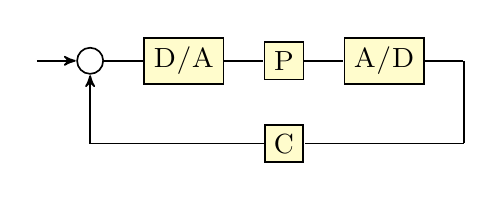
\begin{tikzpicture}[scale=0.3,-,>=stealth',shorten >=.2pt,auto,
     semithick, initial text=, ampersand replacement=\&,]

  \matrix[nodes={draw, fill=none, shape=rectangle, minimum height=.2cm, minimum width=.2cm, align=center}, row sep=.5cm, column sep=.5cm] {
   \coordinate (aux0);
   \& \node[circle] (circle) {}; 
   \& \node[fill=yellow!20] (da) {{\sc D/A}}; 
   \& \node[fill=yellow!20] (p) {{\sc P}};
   \& \node[fill=yellow!20] (ad) {{\sc A/D}}; 
   \& \coordinate (aux1);\\
   \& \coordinate (aux3); 
   \&
   \&
   \node[fill=yellow!20] (c) {C};
   \& 
   \& \coordinate (aux2);\\
  };


  \path[->] (aux0) edge (circle.west);
  \path  
   (circle.east) edge (da.west)
   (da.east) edge (p.west)
   (p.east) edge (ad.west)
   (ad.east) edge (aux1.west)
   (aux1.south) edge (aux2.north)
   (aux2.west) edge (c.east)
   (c.west) edge (aux3.east); 
  \path[->]  (aux3.north) edge (circle.south);
 \end{tikzpicture}
}
 \caption{Closed-Loop System. \label{fig:closed-system}}
\end{figure}

%%%%%%%%%%%%%%%%%%%%%%%%%%%%%%%%%%%%%%%%%%%%%%%%%%%%%%%%%%%%%%%%%%%%%%%%%%%%%%%%%%%%%%
\section{Preliminaries}

\blue{Please insert a figure clearly distinguishing between continuous and discretised/quantised plant - a template is in a picture sent out by Lucas late last week. Please introduced signals on the plot. 

Let us straighten the notations next. 
We should have 
\begin{itemize}
\item 
$G(s) = \frac{s^{M_G}b_{0}+s^{M_G-1}b_{1}+...+b_{M_G}}{s^{N_G}a_{0}+s^{N_G-1}a_{1}+...+a_{N_G}}$ -- this is the physical plant, which is focus of interest and to which we refer our specifications/properties 
\item 
$G(z, T) = \frac{\bar b_{0}+\bar b_{1}z^{-1}+...+\bar b_{M_G}z^{-M_G}}{\bar a_{0}+\bar a_{1}z^{-1}+...+\bar a_{N_G}z^{-N_G}}$ -- this is the time-discretised plant (notice the notation encompasses explicitly the sample time $T$; please write out explicitly the relationship between the $a_i$ and the $\bar a_i$ and likewise for the numerator's coefficients 
(in particular, are the orders $M_G, N_G$ the same? 
\item 
we have $Y(z) = G(z,T) U(z)$; then, we introduce $\hat Y(z) \doteq Y(z) + \nu (z)$, so that 
$$
\frac{\hat Y(z)}{U(z)} = G(z,T) + \frac{\nu (z)}{U(z)} = G(z,T) + \Delta G_Q(z) \doteq \hat G(z) ,  
$$ 
where $\Delta G_Q(z)$ is an error term accounting for the quantisation effects 
\item 
finally, we encompass the errors resulting from employing finite parameters representation, 
which we encompass in a term $\Delta G_P(z)$: is this error additive, so that we would get to a 
$$
\tilde G(z) \doteq \hat G(z) + \Delta G_P(z) = G(z,T) + \Delta G_Q(z) + \Delta G_P(z)?  
$$ 
Dario, can you write it out explicitly? In other words, if 
$$
\hat G(z) = G(z,T) + \Delta G_Q(z) = \frac{\hat b_{0}+\hat b_{1}z^{-1}+...+\hat b_{M_G}z^{-M_G}}{\hat a_{0}+\hat a_{1}z^{-1}+...+\hat a_{N_G}z^{-N_G}},  
$$ 
then what is the explicit expression of 
$$
\tilde G(z) = \frac{\tilde b_{0}+\tilde b_{1}z^{-1}+...+\tilde b_{M_G}z^{-M_G}}{\tilde a_{0}+\tilde a_{1}z^{-1}+...+\tilde a_{N_G}z^{-N_G}}?
$$
(Notice that the orders $M_G, N_G$ need to be properly taken care of.)
\item 
Now, it's over the transfer function $\tilde G(z)$ that we want to synthesise the parameters of a template $C(z)$. 
This controller's transfer function will be subject to the same quantisation and precision limits as the plant's: 
we need to argue that the way we do synthesis affects manipulation of quantities that relate to specific errors and be explicit about these. 
\item[]
\item 
An additional source of error can be related to the fact that a plant transfer function, 
per se a physical entity, is actually represented in a program imprecisely: 
this would mean that $G(s)$ is actually 
$$
G^\ast (s) \doteq \frac{s^{M_G^\ast}b_{0}+s^{M_G^\ast-1}b_{1}+...+b_{M_G}}{s^{N_G^\ast}a_{0}+s^{N_G^\ast-1}a_{1}+...+a_{N_G}}, 
$$ 
which perhaps can indeed be re-written as $G^\ast (s) = G(s) + \Delta G_P(s)$? (This proof should come from that above.) 
We should argue that this error is encompassed by the one derived above (or isn't it?). 
\end{itemize}
}

%------------------------------------
\subsection{Verifying Closed-loop Control Systems}
\label{verifying-closed-loop-control-systems}
%------------------------------------

\red{[This section and the next should be merged into a crisp section with the background on DSVerifier, if not included in previous work? 
Please stick to the introduced notations. Please clarify what the function FWL does, compared to the general approximations introduced above.]}

In this study, the methodology used for verifying closed-loop digital
control system is based on the Digital-System Verifier
(DSVerifier)~\cite{IsmailBCFF15}, which checks the stability of control
systems considering finite-word length (FWL) effects in the digital
controller and uncertainty parameters in the plant model (plant
intervals)~\cite{Bessa16}.  Let $C(z)$ be a digital controller and $G(z)$ be
a plant model given as
%
\begin{align}
\small
\label{controller_plant_tf}
C(z)&=\frac{\beta_{0}+\beta_{1}z^{-1}+...+\beta_{M_C}z^{-M_C}}{\alpha_{0}+\alpha_{1}z^{-1}+...+\alpha_{N_C}z^{-N_C}}, \\
%\label{plant_tf}
G(z)&=\frac{b_{0}+b_{1}z^{-1}+...+b_{M_G}z^{-M_G}}{a_{0}+a_{1}z^{-1}+...+a_{N_G}z^{-N_G}}.
\end{align}
%
\noindent where $\beta$ and $\alpha$ are the controller's coefficients, $b$
and $a$ are the plant's coefficients, and $N$ and $M$ are the number of bits
of the integer and fractional part, respectively.  Note that $G(z)$ is a
discrete model of a real (and continuous) plant, {\it i.e.}, a continuous
model of the plant must be discretized to obtain the discrete equivalent
coefficients $b$ and $a$~\cite{Astrom08} via ZOH discretization %\red{[pls say how]}
. Although there are several discretization methods available in the literature~\cite{Franklin15}, the
zero-order hold (ZOH) discretization is more suitable for representing the
sampling processes that are typically employed by hybrid
systems~\cite{istepanian2012digital} 
\red{[but the ZOH is for the DAC, not for the ADC?]}.

Let $C(z)$ and $G(z)$ transfer functions be arranged in vectors $c_0$ and
$g_0$, respectively.  For each $C(z)$ implementation, there is a function
$\mathit{FWL}[\cdot]:\mathbb{R}^{N_C+M_C}\rightarrow
Q[\mathbb{R}^{N_C+M_C}]$, which applies FWL effects to the controller
$C(z)$, where $Q[\mathbb{R}]$ represents the quantized set of representable
real numbers in the chosen implementation format \param{N_C}{M_C} \red{[clarify this notation]}.  The
quantized controller parameters vector ($c$) is generated via
$\mathit{FWL}[c_0]$.  The uncertain plant parameters ($g$) can be expressed
as
%
\begin{equation}
g = g_0 + \Delta{g} = \left [
				\begin{tabular}{c}
				$b_{0}+\Delta{b_{0}} ~ b_{1}+\Delta{b_{1}} ~ ... ~ b_{M_G}+\Delta{b_{M_G}}$ \\%~ 
				$a_{0}+\Delta{a_{0}} ~ a_{1}+\Delta{a_{1}} ~ ... ~ a_{N_G}+\Delta{a_{N_G}}$
				\end{tabular}
				\right ],
\end{equation}
 
\vspace{1 mm} 
\noindent where $\Delta{g}$ represents the plant uncertainties coefficients. The polynomial set of possible values of $g$ is denoted by $\mathfrak{G}$.

%------------------------------------
\subsection{DSVerifier Verification Flow}
\label{verification-flow}
%------------------------------------

\red{[The following description can be made shorter, crisper?]}

The DSVerifier verification flow is illustrated in
Fig.~\ref{DSVerifier_process}.  Steps $1$ to $5$ are performed by users and
Steps A to D are automatically performed by DSVerifier, which accepts the
digital controller transfer functions together with the plant model.  For
any digital controller, implementation details should be provided ({\it
e.g.}, number of bits, realization, and sample time).

\begin{figure*}[t]
\centering
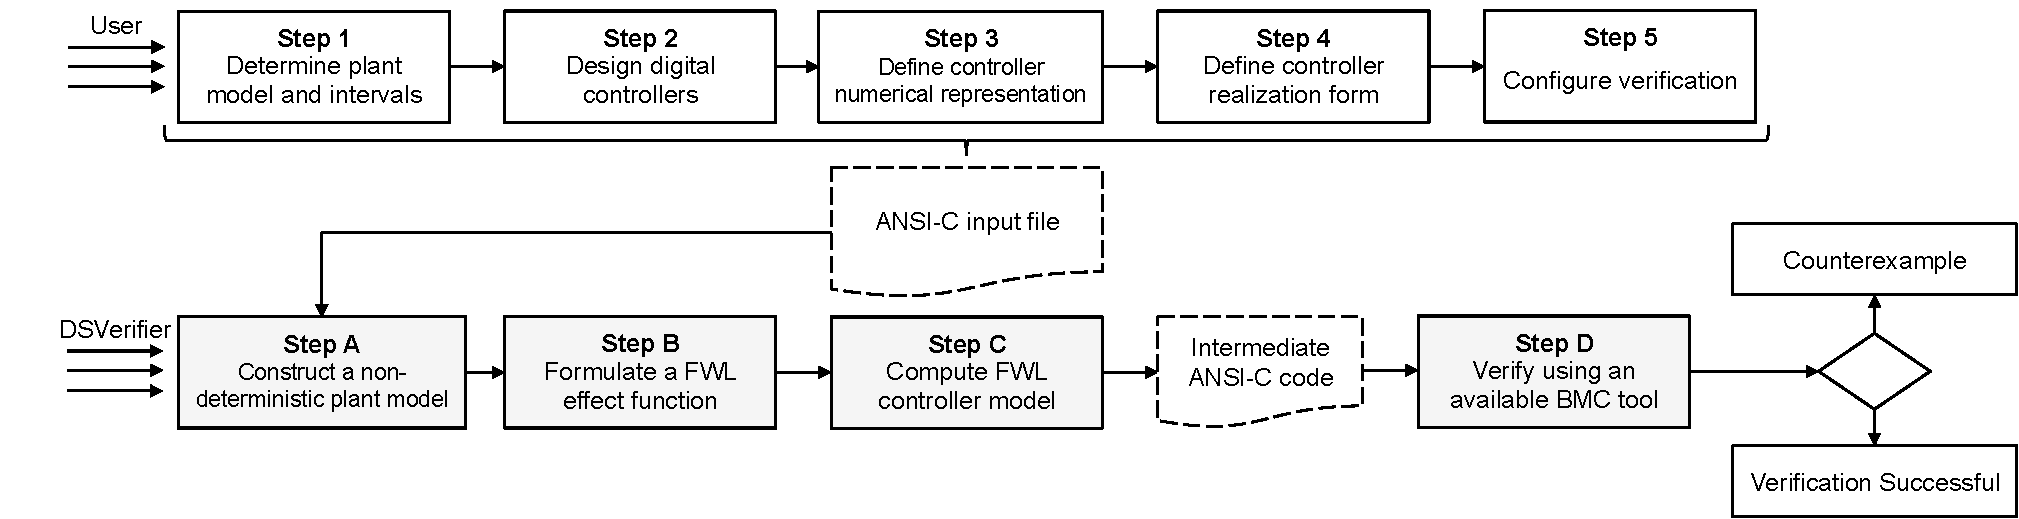
\includegraphics[width=\textwidth]{figures/verification-flow.pdf}
\caption{DSVerifier Verification Flow.}
\label{DSVerifier_process}
\end{figure*}

In Step $1$, the user provides inputs $g_0$ and $\Delta{g}\%$ ({\it i.e.},
percentage form of $\Delta{g}$), which contain the plant model and the
interval, respectively.  In Step $2$, a digital controller must be designed
with any preferred method, where $c_0$ is obtained.  The controller
numerical representation and realization form are chosen in Steps $3$ and
$4$, respectively.  In Step $5$, the user finally configures the
verification parameters ({\it e.g.}, verification time, properties, and BMC
tool).  After that, DSVerifier verification engine performs an (automatic)
verification of the desired property $\phi$ ({\it i.e.}, stability).  The
user steps described in Steps $1$--$5$ result in an ANSI-C code that should
be used as an input for DSVerifier.

In Step A, DSVerifier constructs a non-deterministic model to represent the
plant family $\mathfrak{G}$ using $g_0$ and $\Delta{g}\%$, which are
provided in Step $1$.  DSVerifier then formulates $\mathit{FWL}[\cdot]$ in
Step B using implementation details provided from Steps $2$ and $3$, and
then computes $\mathit{FWL}[c_0]$ in Step C.  Thus, DSVerifier builds an
intermediate ANSI-C code for the digital system implementation, which is
used as input for the model-checker, as pointed in Step D.

This intermediate ANSI-C code model has three main modules: digital
controller code to be embedded into the microprocessor; plant model code,
which simulates the plant model dynamics considering uncertainties; and
``assert'' and ``assume'' statements, which control the verification flow. 
For the digital controller code, transfer functions coefficients are
quantized and deterministic, and all operations use fixed-point arithmetic. 
\textcolor{red}{In the plant model code, transfer function coefficients are
not quantized, but represented with maximum precision based on float
data-type variables}; they are treated as non-deterministic variables to
support model uncertainties.  The directive ``assume'' bounds
non-deterministic variables, {\it i.e.}, inputs and plant uncertain
coefficients.

Finally in the Step D, the translation of ANSI-C code into SAT/SMT formulae
is done by a back-end model-checking tool ({\it e.g.},
CBMC~\cite{ClarkeKL04} or ESBMC~\cite{CordeiroFM12}).  Here, DSVerifier
symbolically checks a given property $\phi$ with respect to closed-loop
systems, which are composed by $FWL[c_0]$ and every $g$ in $\mathfrak{G}$. 
If any property violation is found, then DSVerifier reports a
counterexample, which contains system inputs or parametric deviations
$\Delta{g}\%$ that lead the system to a failure.  A successful verification
result is reported if the system is safe with respect to $\phi$.  In
particular, the stability verification is complete and sound, since it does
not depend on system outputs and inputs.

%%%%%%%%%%%%%%%%%%%%%%%%%%%%%%%%%%%%%%%%%%%%%%%%%%%%%%%%%%%%%%%%%%%%%%%%%%%%%%%%%%%%%%
\section{A Uncertainty Model for Quantization Error} 
\label{sec:uncertainty-model-quantization-error}

In this study, an uncertain plant model $\hat{G}(z)$ is split into two terms:
%
\begin{equation}
\label{eq:uncertainplant}
\hat{G}(z)=G(z)+\Delta{G(z)},
\end{equation}

\noindent where $G(z)$ is the discretized nominal plant model and
$\Delta{G(z)}$ is the additive uncertainty, which is related to parametric
uncertainties~\cite{Bessa16}.  Here, an uncertainty model to accommodate the
quantization noise effects on $\hat{G}(z)$ is proposed.  As a result,
Eq.~\eqref{eq:uncertainplant} is rewritten as
%
\begin{equation}
\label{eq:uncertainFWLplant}
\hat{G}(z)=G(z)+\Delta{G_{Q}(z)}+\Delta{G_{P}(z)},
\end{equation}

\noindent where $\Delta{G_{Q}(z)}$ represents the quantization uncertainty
model and $\Delta{G_{P}(z)}$ describes the parametric uncertainty model. 
Thus, a model for $\Delta{G_{Q}(z)}$ that can represent the quantization
noise effect in the plant output, and consequently the closed-loop system
output, is proposed.  For convenience, the parametric uncertainties will be
described here.

Consider the closed-loop sampled system in Figure~\ref{fig:sampledsystem},
where $C(z)$ is the digital controller model, whose control output signal is
quantized ($Q2$) and interpolated via a ZOH using digital-to-analog
converter (DAC).  $G(s)$ is the continuous-time model of the plant, from
which output samples are taken and quantized ($Q1$) by means of an
analog-to-digital converter (ADC) synchronized with the DAC.  Each quantizer
($Q1$ and $Q2$) will present some contribution for the total quantization
noise.
%
\begin{figure}[ht]
\centering
\resizebox{.5\textwidth}{!}{
 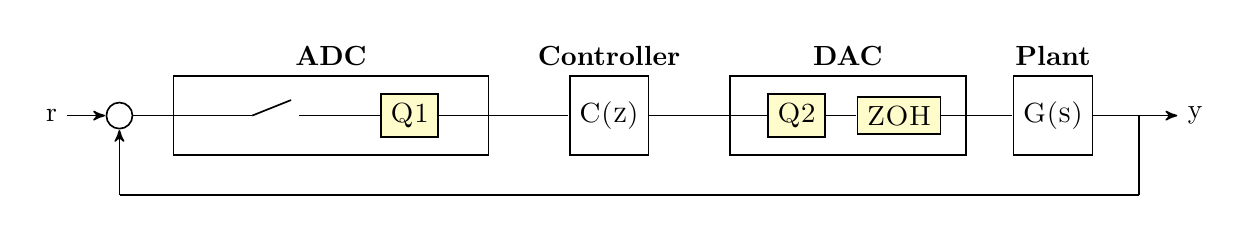
\begin{tikzpicture}[scale=0.3,-,>=stealth',shorten >=.2pt,auto,
     semithick, initial text=, ampersand replacement=\&,]

  \matrix[nodes={draw, fill=none, shape=rectangle, minimum height=.2cm, minimum width=.2cm, align=center}, row sep=.5cm, column sep=.5cm] {
    \node[draw=none] (r) {r};
%   \& \coordinate (aux0);
   \& \node[circle] (circle) {};
   \& complexnode/.pic={ 
     \node[rectangle,draw,
	minimum width=4cm,
	minimum height=1cm,
	label=\textbf{ADC},] (adc) {};
   \draw[] ([xshift=-1cm]adc.center) -- ++(0.5,0.2cm);
   \coordinate (switch1) at ([xshift=-1cm]adc.center);
   \coordinate (switch2) at ([xshift=-0.4cm]adc.center);
   \node[fill=yellow!20] (q1) at ([xshift=1cm]adc.center) {{\sc Q1}};} 
   \& \node[rectangle,draw,
	minimum width=1cm,
	minimum height=1cm,
        label=\textbf{Controller}] (cz) {{\sc C(z)}};
   \& complexnode/.pic={ 
      \node[rectangle,draw,
	minimum width=3cm,
	minimum height=1cm,
	label=\textbf{DAC},] (dac) {};
     \node[fill=yellow!20] (q2) at ([xshift=-.65cm]dac.center) {{\sc Q2}};
     \node[fill=yellow!20] (zoh) at ([xshift=.65cm]dac.center) {{\sc ZOH}};}
   \& \node[rectangle,draw,
	minimum width=1cm,
	minimum height=1cm,
        label=\textbf{Plant}] (gs) {{\sc G(s)}};
   \& \coordinate (aux1);
   \& \node[draw=none] (y) {y};\\
   \& \coordinate (aux3); 
   \&
   \&
   \& 
   \& 
   \& \coordinate (aux2);\\
  };


  \path[->] (r) edge (circle.west);
  \path[->] (aux1) edge (y);
  \path  
   (circle.east) edge (switch1)
   (switch2) edge (q1.west)
   (q1.east) edge (cz.west)
   (cz.east) edge (q2.west)
   (q2.east) edge (zoh.west)
   (zoh.east) edge (gs.west)
   (gs.east) edge (aux1.west)
   (aux1.south) edge (aux2.north)
   (aux2.west) edge (aux3.east); 
  \path[->]  (aux3.north) edge (circle.south);
 \end{tikzpicture}
}
 \caption{Sampled System. \label{fig:sampledsystem}}
\end{figure}


%% \begin{figure}[ht]
%% \centering
%% 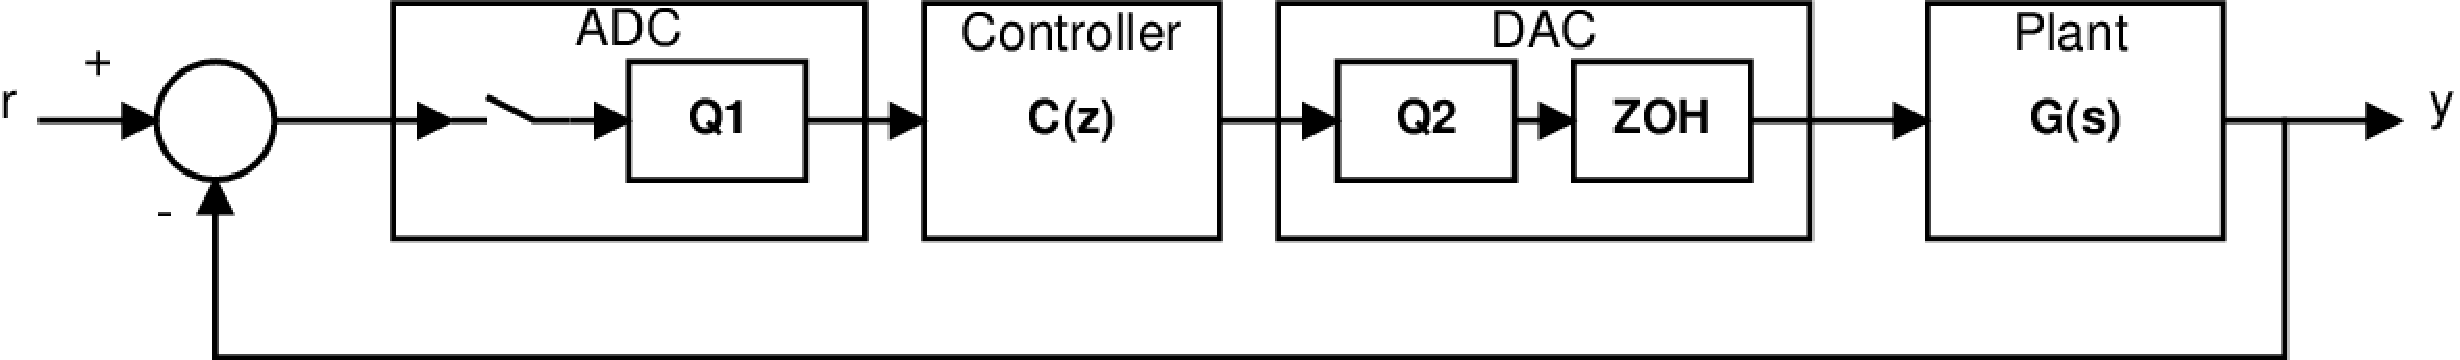
\includegraphics[width=\columnwidth]{figures/hsystembd.pdf}
%% \caption{Sampled system.}
%% \label{fig:sampledsystem}
%% \end{figure}

First, some assumptions have to be established to obtain a model for $\Delta{G_{Q}(z)}$. 
\blue{[Here we need to be careful: we first argue that quantisation (spelled with an s, so that ER II is happy) effects can be represented as an additive noise (great), which however is a stochastic signal. But we handle the noise deterministically. How so? Where is the catch? ]}
%
\begin{myassumption}
\label{whitenoise}
%
The quantization noises $\nu_{1}$ (from the $Q1$) and $\nu_{2}$ (from the
$Q2$) \red{[do we need the second? See my further comments below.]} \green{There was a typo in \eqref{eq:deltaG_final}. It was missing $q_{1}$ and $q_{1}$, both effects are considered here. }
are white noises.
%
\end{myassumption}

\begin{myassumption}
The quantization noises $\nu_{1}$ and $\nu_{2}$ are uncorrelated with each other.
\end{myassumption}

\begin{myassumption}
%
The DAC and ADC are synchronized, {\it i.e.}, there is no delay between
sampling the plant output at ADC and updating the DAC accordingly.
%
\end{myassumption}

\begin{myassumption}
%
The controller and plant are linear, {\it i.e.} any source of nonlinearity ({\it e.g.} overflows) may be disregard. %\red{[explain difference btw overflows and saturations. Also, do we care about limit cycles? I'd quite happily disregard them.]}
%
\end{myassumption}

\begin{myassumption}
%
The DAC interpolator is an ideal ZOH; it takes the discrete value of control
signal $u(k)$ at instant $k$ and produces a rectangular pulse of height
$u(k)$ and width equal to the sample time $T$. \red{[Right: so under this assumption, we really only focus on the quantisation effects introduced by the ADC, correct? Let us not mix up the role and the influence of the two blocks.]}
%
\end{myassumption}

Given those assumptions, the present approach is further based on the following lemmas. 
\red{[So we have introduced two quantisation errors, properly indexed. Next we discuss a non-indexed entity - pls clarify or comment.]}
%
\begin{mylemma}
%
\cite{widrow1956} The second moment (variance) of the probability probability density function of quantization
noise is given by %\textcolor{red}{expand the acronym PDF}
%
\begin{equation}
\label{eq:variancelemma}
\sigma_{Q}^{2}=\frac{q^{2}}{12},
\end{equation}
\end{mylemma}

\noindent where $q$ is the step size of quantizer.

\begin{mylemma} \cite{astrom1997computer}
%
The pulse transfer function $G(z)$ is a z-domain model that relates the output sampled by a ADC and the digital input provided by ZOH. It is equivalent at the sample times ({\it i.e.} $kT$ to the continuous transfer function $G(s)$ driven by ZOH.  This pulse transfer
function can be computed as
%
\begin{equation}
\label{eq:pulsetf}
G(z)=(1-z^{-1})\mathcal{Z}\left\lbrace{\mathcal{L}^{-1}\left\lbrace{\frac{G(s)}{s}}\right\rbrace_{t=kT}}\right\rbrace.
\end{equation}
\end{mylemma}
\red{[Here the dependence on the sampling time T needs to appear somewhere.]} \green{It appears,  $kT$ is the time $t$ used after the inverse Laplace transform}

Considering the quantization noise $\nu(k)$ as an output error in the
discrete plant model, {\it i.e.}, it does not affect the plant dynamics, but
its output samples, it is easy to prove that $\Delta{G_{Q}(z)}$ can be
obtained from
%
\begin{equation}
\label{eq:quantization_tf}
\Delta{G_{Q}(z)}=\frac{\nu(z)}{U(z)},
\end{equation}

\noindent where $\nu(z)$ is the z-transform of the random process $\nu(k)$,
which can be calculated through the power spectral density of
$\nu(k)$~\cite{poularikas2000transforms}.  Thus, the $\Delta{G_{Q}(z)}$ can
expressed as
%
\begin{equation}
\label{eq:deltag_var}
\Delta{G_{Q}(z)}=\frac{\sigma_{Q}^{2}}{U(z)},
\end{equation}

\noindent where $\sigma_{Q}^{2}$ is the variance of the quantization noise and
$U(z)$ is the z-transform of control signal ({\it i.e.}, the z-transform of
the signal from the digital controller), which is provided to the plant by
means of ZOH.

\red{[Please write out a formal statement for the proof below:]}
%
\begin{proof}
%
Suppose that the plant discrete model in Figure~\ref{fig:sampledsystem} can
be represented by the following pulse transfer function (without
quantization noise effect):
%
\begin{equation}
\label{eq:tfwithout}
G(z)=\frac{Y(z)}{U(z)}=\frac{B(z)}{A(z)}=\frac{b_{0}+b_{1}z^{-1}+b_{2}z^{-2}+\cdots+b_{M}z^{-M}}{1+a_{1}z^{-1}+a_{2}z^{-2}+\cdots+a_{N}z^{-N}},
\end{equation}
%
\noindent where $Y(z)$ is the z-transform of the plant output signal without
noise $y(k)$, $U(z)$ is the z-transform of the control signal, which is
provided to the plant, $A(z)$ and $B(z)$ are the plant pulse transfer
function numerator and denominator, respectively.

Considering the quantization noise $\nu(k)$ as an output error in the
discrete plant model, an additive noise in the plant output $y(k)$ resulting
in the noisy output $\hat{y}(k)$ can be represented as
%
\begin{equation}
\hat{y}(k)=y(k)+\nu(k).
\end{equation}

Note that the model in Eq.~\eqref{eq:tfwithout} is equivalent to the
following difference equation:
%
\begin{equation}
\begin{split}
y(k)=-a_{1}y(k-1)-a_{2}y(k-2)-\cdots - a_{N}y(k-N)\\
+b_{0}u(k)+b_{1}u(k-1)+b_{2}u(k-2)+\cdots+b_{M}u(k-M),
\end{split}
\end{equation}

\noindent and consequently $\hat{y}(k)$ can be represented by the following
difference equation:
%
\begin{equation}
\label{eq:differencewithnoise}
\begin{split}
\hat{y}(k)=-a_{1}y(k-1)-a_{2}y(k-2)-\cdots - a_{N}y(k-N)\\
+b_{0}u(k)+b_{1}u(k-1)+b_{2}u(k-2)+\cdots+b_{M}u(k-M)+\nu(k).
\end{split}
\end{equation}

The z-transform of Eq.~\eqref{eq:differencewithnoise} is
%
\begin{equation}
\begin{split}
\hat{Y}(z)=(-a_{1}z^{-1}-a_{2}z^{-2}-\cdots-a_{N}z^{-N})Y(z)\\
+(b_{0}+b_{1}z^{-1}+b_{2}z^{-2}+\cdots+b_{M}z^{-M})U(z)+\nu(z),
\end{split}
\end{equation}
dividing both sides by $U(z)$, it is equivalent to:
\begin{equation}
\frac{\hat{Y}(z)}{U(z)}=\hat{G}(z)=[1-A(z)]G(z)+U(z)B(z)+\frac{\nu(z)}{U(z)}.
\end{equation}

Considering $\hat{G}(z)=G(z)+\Delta{G_{Q}(z)}$ and Eq.~\eqref{eq:tfwithout},
the intended expression can be obtained as
%
\begin{equation}
\Delta{G_{Q}(z)}=\frac{\nu(z)}{U(z)} 
\end{equation}
\end{proof}

Eq.~\eqref{eq:deltag_var} indicates that the modelling of the quantization noise
effect on the plant transfer function demands an estimation of the variance
of quantization noise $\sigma_{Q}^{2}$.  To obtain such estimation, the
methodology presented by~\cite{widrow2008quantization}
is used.  The authors provide an algorithm for computing the mean square of
the output noise due to $Q1$ and $Q2$.  Considering that each quantizer
contribution can be represented by a white noise with zero mean
(Assumption~\ref{whitenoise}), the mean square can be considered as the
variance of noise ($\sigma_{Q}^{2}$), which can be calculated as
%
\begin{equation}
\sigma_{Q}^{2}=\frac{\lambda_{1}^{2}\cdot \sum {h_{Q1}^{2}} \cdot q_{1}+\lambda_{2}^{2}\cdot \sum {h_{Q2}^{2}} \cdot q_{2}}{12},
\end{equation}
%
\noindent where $\lambda_{1}$ and $\lambda_{2}$ are the scale factors \red{[define scale factors]} for the
quantization $Q1$ and $Q2$, respectively; $q_{1}$ and $q_{2}$ are the quantization step for $Q1$ and $Q2$, respectively, and $\sum {h_{Q1}^{2}}$ and $\sum
{h_{Q2}^{2}}$ are the squares sums of the impulse response obtained by means
of a transfer function from $Q1$ and $Q2$ to the plant output, respectively.

The transfer functions $H_{Q1}(z)$ and $H_{Q2}(z)$, from which the squares
sums of the impulse response are needed, can be obtained through the
analysis of the system in Figure~\ref{fig:sampledsystem}.  Considering that
the quantizer $Q1$ is the source of a white noise with zero mean $\nu_{1}$
and $Q2$ is the source of a white noise with zero mean $\nu_{2}$, the
following equation can be written for the system in
Figure~\ref{fig:sampledsystem}
%
\begin{equation}
\resizebox{0.48\textwidth}{!}{
$\hat{Y}(z)=\nu_{1}(z)C(z)G(z)+\nu_{2}(z)G(z)+R(z)C(z)G(z)-\hat{Y}(z)C(z)G(z),$
}
\end{equation}

\noindent which can be rewritten as
%
\begin{equation}
\label{eq:outputfunctions}
\resizebox{0.48\textwidth}{!}{
$\hat{Y}(z)=\frac{C(z)G(z)}{1+C(z)G(z)}R(z)+\frac{C(z)G(z)}{1+C(z)G(z)}\nu_{1}(z) \\
+\frac{G(z)}{1+C(z)G(z)}\nu_{2}(z).$
}
\end{equation}

Thus, $H_{Q1}(z)$ and $H_{Q2}(z)$ can be extracted from Eq.~\eqref{eq:outputfunctions}:
\begin{equation}
H_{Q1}(z)=\frac{C(z)G(z)}{1+C(z)G(z)},
\end{equation}
and
\begin{equation}
H_{Q2}(z)=\frac{G(z)}{1+C(z)G(z)}.
\end{equation}

These equations are sufficient for computing $\sigma_{Q}^{2}$.  However,
there is still a gap for a complete model for $\Delta{G_{Q}(z)}$ in
Eq.~\eqref{eq:deltag_var}, {\it i.e.}, the z-transform of control action
$U(z)$.  This indicates that the quantization noise effect on a discrete
plant model mainly depends on three main factors:
%
\begin{itemize}
%
\item \textbf{Sample time:} the sample time effect is reflected over pulse transfer function that covers the effects of DAC ant its interpolator (ZOH) \red{[clarify/revise based on the comments made above.]};
%
\item \textbf{ADC and DAC step:} \red{[again, do we need both?]} these are the main component of quantization noise power, but an $8$-bits converter already reduces the effect of quantization noises in the output for negligible values.
%
\item \textbf{Signal-to-noise ratio (SNR): } the dependence on the value of $U(z)$ \red{[notice that now we have reduced the problem to depend on the effect of the reference signal transform R(z) - pls revise.]} shows the importance of the SNR for handling quantization noise; for a high SNR of the digital controller, the quantization effect is negligible. This happens during the transient of the system, when high control actions are employed. However, it can be relevant during the steady state. A digital controller with integral action might be sufficient for eliminating such influence at steady state.
%
\end{itemize}

An alternative expression for $\Delta{G_{Q}(z)}$ can be obtained from
Eq.~\eqref{eq:deltag_var}, transforming it into a function of the reference
$R(z)$.  Once $U(z)$ is the control signal obtained via digital controller
$C(z)$ and error signal, {\it i.e.},
%
\begin{equation}
U(z)=C(z)\cdot[R(z)-Y(z)],
\end{equation} 

\noindent where $Y(z)$ is the first term of Eq.~\eqref{eq:outputfunctions}, thus:
\begin{equation}
\label{eq:controlsignal}
\resizebox{0.48\textwidth}{!}{
$U(z)=C(z)\cdot \left[R(z)-\frac{C(z)G(z)}{1+C(z)G(z)}R(z)\right]=\frac{C(z)}{1+C(z)G(z)}R(z).$
}
\end{equation} 

Substituting Eq.~\eqref{eq:controlsignal} in Eq.~\eqref{eq:deltag_var}, a
model for $\Delta{G_{Q}(z)}$ depending on $R(z)$ can be obtained:
%
\begin{equation}
\Delta{G_{Q}(z)}=\sigma^{2}_{Q}\cdot \frac{1+C(z)G(z)}{C(z)} \cdot \frac{1}{R(z)},
\end{equation}

\noindent where $R(z)$ can be considered as a step signal (for stabilization
purpose) with height equal to $r$, which can be rewritten as
%
\begin{equation}
\Delta{G_{Q}(z)}=\frac{\sigma^{2}_{Q}}{r}\cdot \frac{1+C(z)G(z)}{C(z)} \cdot \frac{z-1}{z}.
\end{equation}

A more precise description of $\Delta{G_{Q}(z)}$ can be obtained
considering FWL \red{[clarify what you mean with FWL, introduce FWL function explicitly and precisely]} effects on digital controller coefficients, as described in
Bessa {\it et al.}~\cite{Bessa16}, {\it i.e.}, using $FWL[C(z)]$ instead of
the nominal $C(z)$:
%
\begin{equation}
\label{eq:deltaG_final}
\Delta{G_{Q}(z)}=\frac{\sigma^{2}_{Q}}{r}\cdot \frac{1+FWL[C(z)]G(z)}{FWL[C(z)]} \cdot \frac{z-1}{z}.
\end{equation}

Finally, Eq.~\eqref{eq:deltaG_final} is a suitable frequency domain model
for quantization noise effects on closed-loop systems.  This model depends
on the plant pulse transfer function ($G(z)$), which is described by
Eq.~\eqref{eq:pulsetf}, the height of step reference signal $r$, and the
digital controller model.


%%%%%%%%%%%%%%%%%%%%%%%%%%%%%%%%%%%%%%%%%%%%%%%%%%%%%%%%%%%%%%%%%%%%%%%%%%%%%%%%%%%%%%
\section{Running Example} \label{sec:running-ex}

A classical cruise control example is extracted from the
literature~\cite{Astrom08}, where the discrete plant model (with time step
of $0.2$s) is represented by the following z-expression:

\begin{equation}
\label{Eq:running-example-plant}
G\left(z\right) := \frac{0.0264}{z-0.9998}.
\end{equation}

Using an optimization tool, Wang {\it et
al.}~\cite{DBLP:conf/hybrid/WangGRJF16} design a high-performance
controller, which is characterized by the following z-expression:

\begin{equation}
\label{Eq:running-example-controller}
C\left(z\right) := \frac{2.72z^2 - 4.153z + 1.896}{z^2 - 1.844z + 0.8496}.
\end{equation}

The authors claim that this controller $C(z)$ is extremely stable for the
discrete plant model $G(z)$.  However, if implementation aspects are
considered during verification, this controller becomes unstable.

For this particular example, the actual implementation of $C(z)$ using
\param{3}{16} implementation format can be represented by the following
z-expression:

\begin{equation}
\label{Eq:running-example-controller-quantized}
\resizebox{0.5\textwidth}{!}{
$C_{q}\left(z\right) {:=} \frac{4.00888156890869140625z^2{-}0.00041961669921875z
-0.000213623046875}{-0.003753662109375z^2{+}7.37355804443359375z-7.2847900390625},$
}
\end{equation} 


\noindent which makes the system unstable in closed-loop using the typical series loop configuration.

%%%%%%%%%%%%%%%%%%%%%%%%%%%%%%%%%%%%%%%%%%%%%%%%%%%%%%%%%%%%%%%%%%%%%%%%%%%%%%%%%%%%%%
%\section{Error Bound Verification}

%As described in the literature, computation using FWL leads to rounding and truncation errors~\cite{Oppenheim1999}. In the present work, impairments present on a closed-loop  system output, due to coefficient rounding and arithmetic-operation results, are considered. Let $x$ be a real number and $x^*$ be a floating-point representation of $x$. The absolute error $\epsilon$, due to the rounding of $x$ represented in floating-point as $x^*$, is 
%
%\begin{equation} \label{absolute-error}
%x^* = x + \epsilon,
%\end{equation}

%\noindent and the relative error $\delta$ by
%
%\begin{equation} \label{relative-error}
%x^* = x\left(1+\delta\right).
%\end{equation}

%The verification of output error bound is proposed, where the output of a closed-loop system, implemented with reduced-word-length floating-point representation, is compared with a reference output of the same structures, implemented using real variables. 

%Thus, considering that the number of precision bits $l_{d}$ in reference models is higher than in designed models, the quantization error $E_{r}$ is given by
%\begin{equation} \label{errorfixlimits}
%-2^{-l-1} + 2^{-l_{d}-1} \leq E_{r} \leq 2^{-l-1} - 2^{-l_{d}-1}.
%\end{equation}

%The expression above shows that the error, computed with the proposed method, is affected by the precision of the reference model.

%For the reduced floating-point models, the computed values are saturated to the maximum representable number on overflow, or to the minimum on underflow; the same input is applied to both models. The input vector uses non-deterministic values from $\{ 2^{k-1}-2^{-l}, 2^{-l}, 0, -2^{-l}, 2^{k-1} \}$, that is, values for maximum and minimum amplitudes of the input signal. So, errors due to quantization and saturation are explored.

%During closed-loop operation unrolling, the cumulative error can increase beyond the quantization-error interval. The following literal is then generated, in order to check whether the output error is in accordance with an acceptable margin:
%\begin{equation} \label{errorcheck}
%	l_{no\_error} \Leftrightarrow \arrowvert y - y_{d} \arrowvert \leq M \cdot 2^{-l-1},
%\end{equation}

%\noindent where $y$ is the output of the designed system, $y_{d}$ is the output of the double precision system, and $M~2^{-l-1}$ is the tolerance margin. The verification process searches for the negation of this literal. When such a counterexample is found, it indicates that the output error is higher than expected for that controller realization.


%%%%%%%%%%%%%%%%%%%%%%%%%%%%%%%%%%%%%%%%%%%%%%%%%%%%%%%%%%%%%%%%%%%%%%%%%%%%%%%%%%%%%%
\section{Program Synthesis}

% We use CounterExample-Guided Inductive Synthesis (CEGIS), as
% illustrated in Fig~\ref{fig:CEGIS}.

In order to synthesise closed-loop digital control systems, we use a
program synthesis engine.  Nowadays, such engines are used
increasingly often in program verification
\cite{DBLP:conf/cav/0001A14,DBLP:conf/lpar/DavidKL15}.  Our program
synthesiser makes use of Counter-Example Guided Inductive Synthesis
(CEGIS) \cite{sketch}.  We start by presenting its general
architecture followed by describing the parts specific to control
systems.

%specialised it for stream refactoring.  
% adding JST for stream refactoring

\paragraph{General architecture of the program synthesiser}
%
The design of our synthesiser is given in
Fig.~\ref{fig:CEGIS} and consists of two phases, {\sc
Synthesise} and {\sc Verify}, which interact via a finite set of test vectors {\sc inputs}.
The {\sc synth} procedure tries to find an existential witness $P$
that satisfies the specification $\sigma(x, P)$ for all $x$:
%
$\exists P . \forall x \in \text{\sc inputs} . \sigma(x, P)$

If {\sc synthesise} succeeds in finding a witness $P$, this witness is a
candidate solution to the full synthesis formula.  We pass this candidate
solution to {\sc verify} which determines whether it does satisfy
the specification on all inputs by checking satisfiability of the
verification formula:
%
$\exists x . \lnot \sigma(x, P)$

If this formula is unsatisfiable, the candidate solution is in fact a
solution to the synthesis formula and so the algorithm terminates. 
Otherwise, the witness $x$ is an input on which the candidate solution fails
to meet the specification.  This witness $x$ is added to the {\sc inputs}
set and the loop iterates again.  It is worth noting that each iteration of the
loop adds a new input to the set of inputs being used for synthesis.  If
the full set of inputs is finite, this means that the refinement loop
can only iterate a finite number of times.

\paragraph{Elements specific to control systems}
Next, we describe the specific property that we pass to the 
program synthesiser as the specification $\sigma$.
There are two different algorithms in DSVerifier that can be used for
stability verification, one based on Schur's decomposition and another
one based on Jury's criteria \cite{DBLP:journals/dafes/BessaICF16}.
Here, we choose Jury's method due to its efficiency.

Essentially, we use this method to check the stability in the $z$-domain
for the characteristic polynomial $S(z)$ of 
the matrix $\left( \begin{array}{c} Y \\ U \end{array}\right)$.
We consider the following form for $S(z)$:
%
$$
S(z) = a_0Z^N+a_1z^{N-1}+\cdots+a_{N-1}z+a_N=0, a_0\neq0
$$
%
%\cdsay{is this for the matrix $\left( \begin{array}{c} Y \\ U \end{array}\right)$?}

Next, the following Jury matrix
$M = [m_{ij}]_{(2N−2)\times N}$ is built from $S(z)$ coefficients:
%
$$
M=\left( 
\begin{array}{c}
V^{(0)}\\
V^{(1)}\\
\vdots\\
V^{(N-2)}
\end{array}
\right)
$$
%
where $V^{(k)} = [v^{(k)}_{ij} ]_{2\times N}$ such that:
%
$$
v_{ij}^{(0)}=\left\{
\begin{array}{ll}
a_{j-1}, & \texttt{if}~i=1\\
v_{(1)(N-j+1)}^{0},&\texttt{if}~i=2
\end{array}
\right.
$$
%
$$
v_{ij}^{(k)}=\left\{
\begin{array}{ll}
0,&\texttt{if}~j>n-k\\
v_{1j}^{(k-1)}-v_{2j}^{(k-1)} . \frac{v_{11}^{(k-1)}}{v_{21}^{(k-1)}}, & \texttt{if}~j\leq n-k ~\texttt{and}~i=1\\
v_{(1)(N-j+1)}^{k},& \texttt{if}~j\leq n-k ~\texttt{and}~i=2\\
\end{array}
\right.
$$
%
where $k \in \mathbb{Z}$, such that $0 < k < N - 2$. 
$S(z)$ is the
characteristic polynomial of a stable system if and only if
the following four propositions hold:
\begin{itemize}
\item $R_1: S(1) > 0$;
\item $R_2: (−1)^N S(−1) > 0$;
\item $R_3: |a_0| < a_N$;
\item $R_4: m_{11} > 0 \wedge m_{31}>0 \wedge m_{51}>0 \wedge \cdots \wedge m_{(2N{-}3)(1)}>0$.
\end{itemize}

The stability property is then encoded by creating a
constraint of the form:
$$\phi_{stability} \equiv (R_1 \wedge R_2 \wedge R_3 \wedge R_4)$$
%\cdsay{figure out what is existentially quantified for the final $\sigma$.}

In the {\sc verify} phase, if the system is unstable for the current candidate solution,
i.e. if $\neg \phi_{stability}$ is satisfiable for $S(z)$, 
then we obtain a counterexample denoted by 
values for each coefficients of $\Delta N_{G}(z)$ and $\Delta D_{G}(z)$,
which make the closed-loop system unstable. This uncertainty is added to 
the set {\sc inputs} such that, in the subsequent {\sc synthesise} phase, 
we obtain a candidate solution consisting 
of a controller $D_C$ and $N_C$, which makes the closed-loop 
system stable for all the uncertainties accumulated in {\sc inputs}.

\paragraph{Using the program synthesiser for the running example}
We will illustrate our synthesis approach on the running example 
in Sec.~\ref{sec:running-ex}.
We start with a candidate solution that has all coefficients 0.
In the first {\sc verify} phase we obtain the following counterexample:
$$
\begin{array}{ll}
\Delta N_G(z) = 0.02634525299072265625\\
\Delta D_G(z) = 0.9979267120361328125z-0.99768829345703125
\end{array}
$$

We add this counterexample to {\sc inputs} and initiate the {\sc
  synthesise} phase, where we get the following candidate solution:

$$
\begin{array}{ll}
N_C(z) {=} 4.00888156890869140625z^2{-}0.00041961669921875z\\
\qquad\qquad -0.000213623046875\\
D_C(z) {=} -0.003753662109375z^2{+}7.37355804443359375z \\
\qquad\qquad -7.2847900390625\\
\end{array}
$$

In the second {\sc verify} phase, we check whether the current candidate
solution above is the final solution. It is not and we get a new counterexample:
$$
\begin{array}{ll}
\Delta N_G(z) = 0.02644824981689453125\\
\Delta D_G(z) {=} 1.00053310394287109375z{-}1.0014629364013671875
\end{array}
$$

After adding this new counterexample to the set of {\sc inputs}, in the 
next {\sc synthesise} phase, we get a new candidate solution that holds
for both uncertainties in {\sc Inputs}:

$$
\begin{array}{ll}
N_C(z) {=} 7.515781402587890625z^2{-}4.385616302490234375z\\
\qquad\qquad +4.142093658447265625\\
D_C(z) {=} -3.52398681640625z^2{-}1.530254364013671875z \\
\qquad\qquad +7.58094024658203125\\
\end{array}
$$

This candidate solution is validated as the final solution by the next 
{\sc verify} phase, which fails to find a new counterexample (i.e. returns UNSAT).

% Counterexample from first cruisecontrol02.c benchmark with uncertainty and
% nondeterminism:
% 1) { (0.02634525299072265625, 0.9979267120361328125, -0.99768829345703125) }

% 2) { (0.02644824981689453125, 1.00053310394287109375, -1.0014629364013671875) }

% <a>
% <item>7.515781402587890625</item>
% <item>-4.385616302490234375</item>
% <item>4.142093658447265625</item>
% </a>
% <a_size>3</a_size>
% <b>
% <item>-3.52398681640625</item>
% <item>-1.530254364013671875</item>
% <item>7.58094024658203125</item>
% </b>
% <b_size>3</b_size>

\begin{figure*}
\centering
\resizebox{.7\textwidth}{!}{
 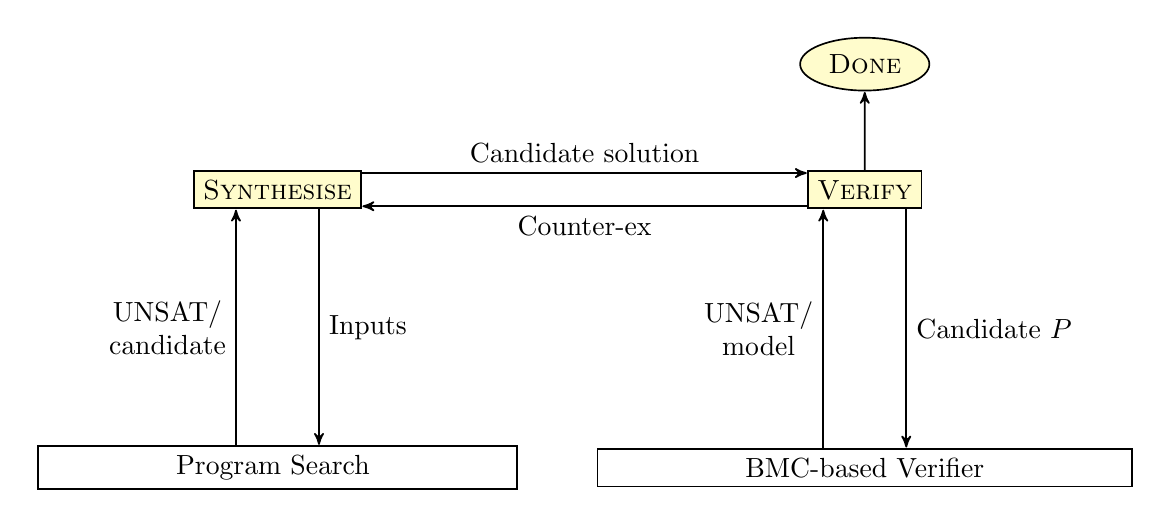
\begin{tikzpicture}[scale=0.3,->,>=stealth',shorten >=.2pt,auto, semithick, initial text=, ampersand replacement=\&,]
  \matrix[nodes={draw, fill=none, shape=rectangle, minimum height=.2cm, minimum width=.2cm, align=center
},
          row sep=1cm, column sep=1cm] {
   \& \node[ellipse, fill=yellow!20] (done) {{\sc Done}}; \\
   \node[fill=yellow!20] (synth) {{\sc Synthesise}};
   \&
   \node[fill=yellow!20] (verif) {{\sc Verify}}; \\

   \& \\
   \& \\
   \node (gp) {~~~~~~~~~~~~~~Program Search~~~~~~~~~~~~~~~};
   \&
   \node (bmc) {~~~~~~~~~~~~~~~BMC-based Verifier~~~~~~~~~~~~~~~};
   
    \\
  };

   \path
    ([yshift=2em]synth.east) edge node {Candidate solution} ([yshift=2em]verif.west)
    ([yshift=-2em]verif.west) edge node {Counter-ex} ([yshift=-2em]synth.east)
    ([xshift=5em]verif.south) edge node {Candidate $P$} ([xshift=5em]bmc.north)
    ([xshift=-5em]bmc.north) edge node[align=center]  {UNSAT/\\model} ([xshift=-5em]verif.south)
    (verif) edge node {} (done)
    ([xshift=5em]synth.south) edge node[align=center] {Inputs} ([xshift=5em]gp.north)
    ([xshift=-5em]gp.north) edge node[align=center] {UNSAT/\\candidate} ([xshift=-5em]synth.south);
 \end{tikzpicture}
}
 \caption{Counterexample-Guided Inductive Synthesis. \label{fig:CEGIS}}
\end{figure*}
%%%%%%%%%%%%%%%%%%%%%%%%%%%%%%%%%%%%%%%%%%%%%%%%%%%%%%%%%%%%%%%%%%%%%%%%%%%%%%%%%%%%%%
\section{Experimental Evaluation}

This section is split into three parts. Section~\ref{experimental-objectives} describes the experimental objectives, while Section~\ref{experimental-setup} discusses the experimental setup and the employed benchmarks. Section~\ref{experimental-results} describes the experimental results related to the application of CEGIS to standard control system benchmarks extracted from the literature.

%---------------------------------
\subsection{Objectives}
\label{experimental-objectives}
%---------------------------------

%---------------------------------
\subsection{Description of Benchmarks}
\label{experimental-setup}
%---------------------------------

The first set of benchmarks considers the discrete plant of a cruise 
control model for the car accounting for rolling friction, aerodynamic drag, 
and gravitational disturbance force~\cite{Astrom08} as follows
%
\begin{equation}
\label{cruise-control-c1}
G_1(z)=\frac{0.0264}{z-0.998}. \nonumber
\end{equation} 

Two proportional-integral (PI) controllers are designed by Wang {\it et al.} 
for the cruise control plant $G(z)$~\cite{DBLP:conf/hybrid/WangGRJF16}, 
which has the following mathematical model
%
\begin{equation}
\label{cruise-control-g1}
C_{1}(z)=\frac{1.51z-1.3586}{z-1}, \nonumber
\end{equation} 
%
\begin{equation}
\label{cruise-control-g2}
C_{2}(z)=\frac{2.72z^2 - 4.153z + 1.896}{1.0z^2 - 1.844z + 0.8496}. \nonumber
\end{equation} 

The second set of benchmarks considers a simple spring-mass 
damper~\cite{DBLP:conf/hybrid/WangGRJF16}, where both discrete 
plant dynamics and controller are represented by the following 
z-expression, resp.
%
\begin{equation}
\label{spring-mass-damper-g}
G_2(z)=\frac{5\times{10^{-5}}z + 5\times{10^{-5}}}{z^2 - 2z + 1.0001}, \nonumber
\end{equation} 
%
\begin{equation}
\label{spring-mass-damper-c}
C_3(z)=\frac{1.28\times{10^{3}}z^2 - 1.354240\times{10^{3}}z + 0.074879\times{10^{3}}}{z^2 - 1.4990z + 0.4995}. \nonumber
\end{equation} 


All experiments were conducted on an otherwise idle Intel Core i$7$-$4790$ 
CPU $3$.$60$ GHz, $16$ GB of RAM, and Linux OS.  All times given are wall 
clock time in seconds as measured by the UNIX time command.

%---------------------------------
\subsection{Results}
\label{experimental-results}
%---------------------------------

%%%%%%%%%%%%%%%%%%%%%%%%%%%%%%%%%%%%%%%%%%%%%%%%%%%%%%%%%%%%%%%%%%%%%%%%%%%%%%%%%%%%%%
\section{Related Work}

\paragraph{Robust synthesis of Linear Systems} 

The problem of parametric control synthesis based on stability measures for
continous Linear Time Invariant (LTI) Single Input-Single Output (SISO)
systems has been researched for several decades.  On a theoretical level it
is a solved problem~\cite{wonham1967pole} for which researches continuously
seek better results based on a number of properties in addition to
stability.  A vast range of pole placement techniques such as Moore's
algorithm for eigenstructure assignment~\cite{klein1977eigenvalue} or the
more recent Linear Quadratic Regulator (LQR)~\cite{bemporad2002explicit}
have been used in several papers with increasing degrees of succes to ensure
stability.  The latter approach highlights the importance of conserving
energy during the control process, which results amongst other things in
lower running costs.  Since real systems are subject to tolerance and noise
as well as the need for economy, more recent works focus on the problems of
achieving robust stability with minimum
gain~\cite{schmid2014unified,konigorski2012pole}.  However, when extending
the problem to digital controller synthesis, many of these techniques lack
the ability to produce sound or stable results because they disregard the
effects of quantization and rounding.  Modern papers on
implementations/synthesis of LTI digital
controllers~\cite{das2013lqr,ghosh2013fpga} focus on time discretization,
failing to account for these error-inducing effects and can therefore result
in digitally unstable systems that have been proven to be robustly stable in
a continuous space.  This situation demands the inclusion of formal methods
to verify the effects of space discretization on the implementation of the
controller.

\paragraph{Formal Verification of Linear Digital Controllers} 

Researchers in formal verification methods of control systems have studied
various effects of discretising the dynamics, including delayed
response~\cite{Duggirala2015}, and Finite Word Length (FWL) constraints with
the objective to either verify (eg.  \cite{daes20161}) or optimise
(eg.~\cite{oudjida2014design}) implementations.  There are in fact two
different problems arising from FWL effects.  The first corresponds to the
error in the dynamics caused by the inability of the hardware to represent
the exact dynamics of the system whilst the second relates to rounding
errors during computation.  In \cite{fialho1994stability} a stability
measure based on the error of the digital dynamics ensures that the FWL
errors do not make the digital system unstable.  A more recent
approach~\cite{DBLP:journals/automatica/WuLCC09} uses $\mu$ calculus to
directly model the digital controller so that the selected parameters are
stable by design.  Most papers following this line of verification focus on
finding a correct implementation of a known desired controller, looking for
optimal parameter representations using FWL but ignoring the effects of
rounding errors due to issues of mathematical tractability.  The analyses
in~\cite{DBLP:conf/hybrid/WangGRJF16,DBLP:conf/hybrid/RouxJG15} rely on an
invariant computation on the discrete system dynamics using Semi-Definite
Pogramming (SDP).  Whilst the former uses BIBO properties to determine
stability, the latter uses Lyapunov-based quadratic invariants.  In both
cases the SDP solver uses floating point arithmetic and soundness is checked
by upper bounding the error.
An alternative approach is taken by \cite{park2016scalable}, where the verification of existing
code is performed against a known model by extracting an LTI model of the
code through symbolic execution. In order to account for rounding errors, an
upper bound is introduced in the verification phase. If the error of the implementation
is lower than this tolerance level, then the verification is successful. 

\paragraph{Robust Synthesis of FWL Digital Controllers}

To the authors' knowledge, there is no existing work on the automatic
synthesis of fixed point digital controllers considering FWL effects.  Parameter
synthesis tools such as~\cite{cimatti2013parameter} use bounded model
checking and fixed point computations to find parameters based on user
defined specifications, but they often operate in the continuous domain and
are ill-suited for robust analysis since they have no direct means of
evaluating robustness.  Other tools such as~\cite{economakos2016automated}
are directly aimed at robust stability problems but fail to explore the
effects of FWL in their implementation.  In order to provide a correct by
design controller, \cite{alur2016compositional} requires a user-defined
finite state abstraction to synthesise a digital controller based on high
level specifications.  Whilst this approach directly overcomes the
challenges presented by the FWL problem, it still requires error-prone user
intervention.  A different solution that looks at the other end of the scale
is an approach that synthesises word lengths for know problems as developed
in \cite{jha2013swati}, however this provides neither an optimal word
synthesis nor a comprehensive solution for the problem.  It is from this
vacuum that we seek to explore a CEGIS approach to FWL controller synthesis.

\paragraph{CEGIS}

In recent years the development of program synthesis has found many ways to
obtain correct by design programs from high level specifiactions.  One such
approach~\cite{itzhaky2010simple} looks to inductively synthesise invariants
to generate the desired programs.  Since these digital programs are already
constrained by designed to factors such as FWL, these approaches are ideal
for the synthesis of parametric controllers. 
In~\cite{DBLP:conf/cdc/RavanbakhshS15}, the authors use CEGIS for the
synthesis of switching controllers for stabilizing continuous-time plants
with polynomial dynamics.  The work extends to its application on affine
systems, finding its major challenge in the hardness of solving linear
arithmetic on present SMT solvers.  Since this approach uses switching
states instead of linear dynamics in the digital controller, it entirely
circumvents the FWL problem.  It is also not suitable for the kind of
control we seek to synthesise.  What is needed in this regard is the
combination of a synthesis engine with a control verification tool that
addresses the challenges presented here in the form of FWL effects and
stability measures for LTI SISO controllers.  We take the former
from~\cite{DBLP:conf/lpar/DavidKL15} and the latter from \cite{daes20161} whilst enhancing the
procedure by evaluating the quantaization effects of the Hardware interfaces
(ADC/DAC) to obtain an accurate discrete time FWL representation of the
continuous dynamics.
 
%In \cite{DBLP:journals/corr/PakmehrWJVF13}, Pakmehr et al.  design a control software verification framework for gas turbine engines.

%%%%%%%%%%%%%%%%%%%%%%%%%%%%%%%%%%%%%%%%%%%%%%%%%%%%%%%%%%%%%%%%%%%%%%%%%%%%%%%%%%%%%%
\section{Conclusions}

\bibliographystyle{abbrv}
\bibliography{paper}  

%APPENDICES are optional
%\balancecolumns
%\appendix
%Appendix A
\end{document}
